%!TEX root = ../main.tex

\section{Results and discussion}

This section provides results and related discussions for modeling the effects of different fluidization gases on the operation of a bubbling fluidized bed reactor. Gas effects on the pyrolysis yields of the biomass feedstock are also presented and discussed.

% ----------------------------------------------------------------------------

\subsection{Pure gas properties}

Molecular weight, viscosity, density, thermal conductivity, heat capacity, and the Prandtl number of the individual gases investigated in this paper are shown in Figure \ref{fig:gas-properties}. The gas properties were calculated at a pressure of 101,325 Pa and a temperature of 773.15 K (500$^\circ$C). The lightest gas in terms of molecular weight and density is hydrogen while the heaviest gas is carbon dioxide. The highest viscosity is noted for the nitrogen gas while hydrogen has the lowest viscosity. The largest thermal conductivity is for hydrogen at approximately 0.36 W/m$\cdot$K while the other gases remain below 0.12 W/m$\cdot$K. The highest heat capacity is obtained for methane at 62 J/mol$\cdot$K while the lowest is for hydrogen at 29 J/mol$\cdot$K. The Prandtl number is similar for all the gases except for water vapor.

\begin{figure}[H]
    \centering
    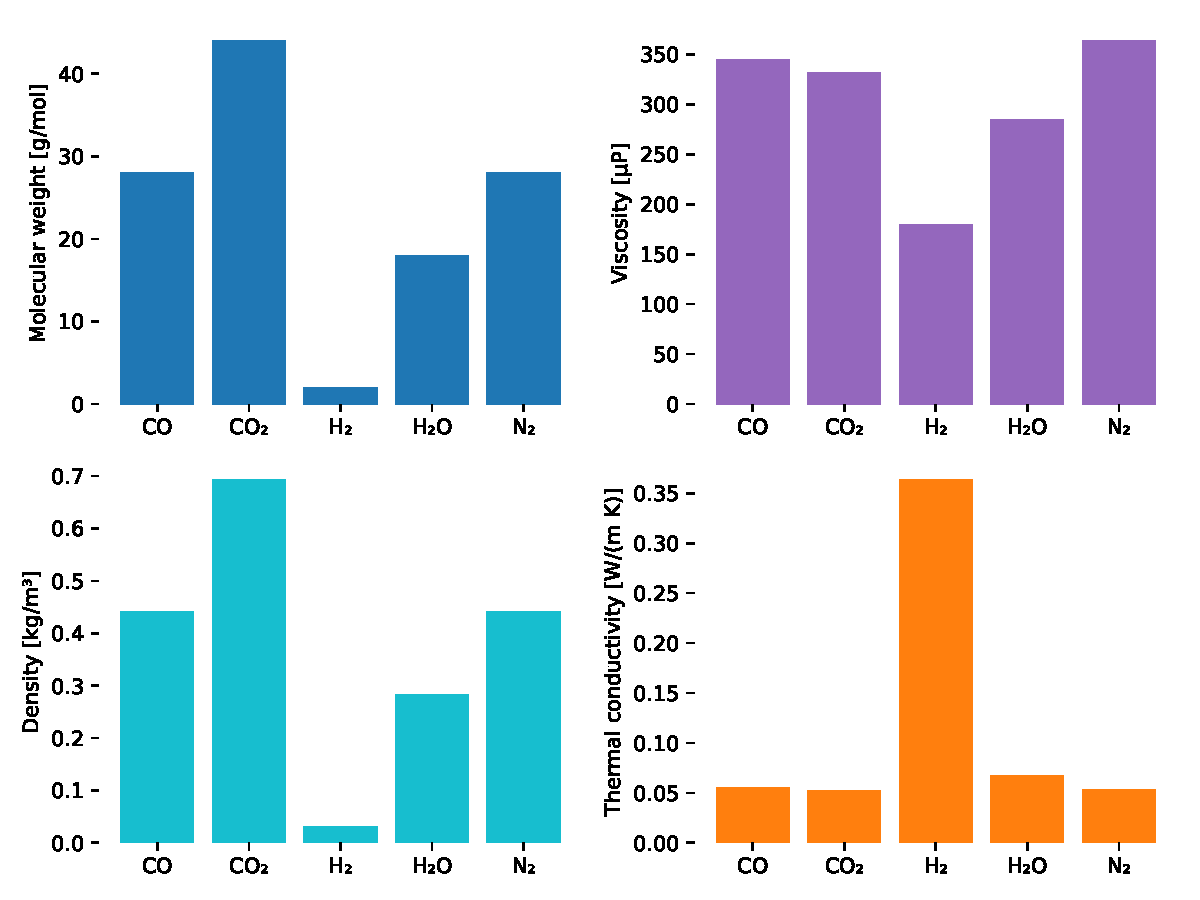
\includegraphics[width=\textwidth]{gas-properties.pdf}
    \caption{Comparison of molecular weight (MW), viscosity ($\mu$), density ($\rho$), thermal conductivity (k), heat capacity (Cp), and Prandtl number (Pr) for each gas at 101,325 Pa and 773.15 K (500$^\circ$C).}
    \label{fig:gas-properties}
\end{figure}

% ----------------------------------------------------------------------------

\subsection{Gas mixture properties}

Comparisons of the calculated viscosity of a H$_2$/N$_2$ gas mixture to measured values obtained from literature are shown in Figure \ref{fig:gas-mu-h2n2-validate}. The models by Herning and Zipperer as well as Brokaw match well with the experimental data for a range of mixture ratios. This is contradictory to the Davidson report which does not recommend the Herning and Zipperer model for hydrogen mixtures \cite{Davidson-1993}. The Davidson and Graham models significantly underpredict the mixture viscosity while the Wilke model tends to overestimate the viscosity. Similar results are obtained for a H$_2$/O$_2$ gas mixture as shown in Figure \ref{fig:gas-mu-h2o2-validate}.

\begin{figure}[H]
    \centering
    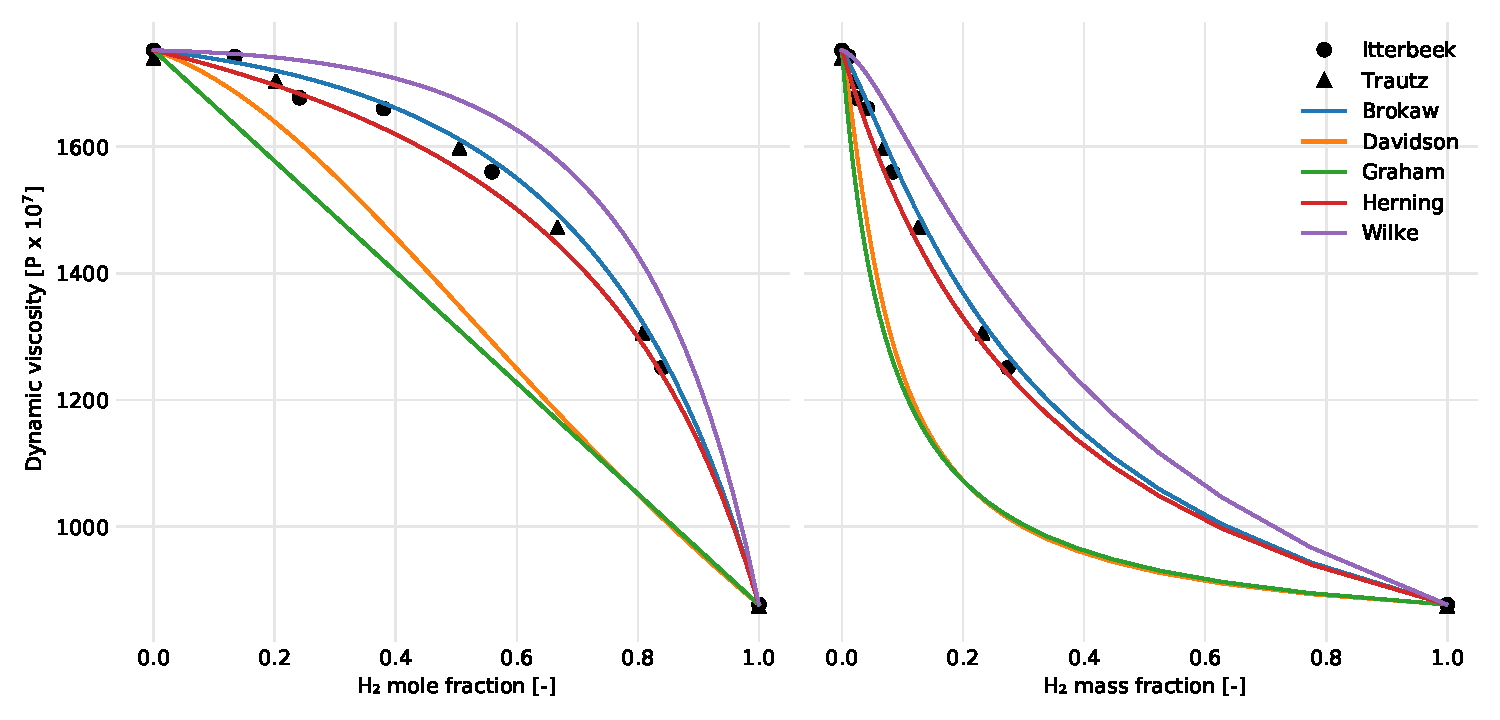
\includegraphics[width=\textwidth]{figures/gas-mu-h2n2-validate.pdf}
    \caption{Viscosity of a H$_2$/N$_2$ mixture at 291.1 K (18$^\circ$C). Calculated values represented by line profiles. Experiment data points from \cite{Itterbeek-1947,Trautz-1929} shown as symbols.}
    \label{fig:gas-mu-h2n2-validate}
\end{figure}

\begin{figure}[H]
    \centering
    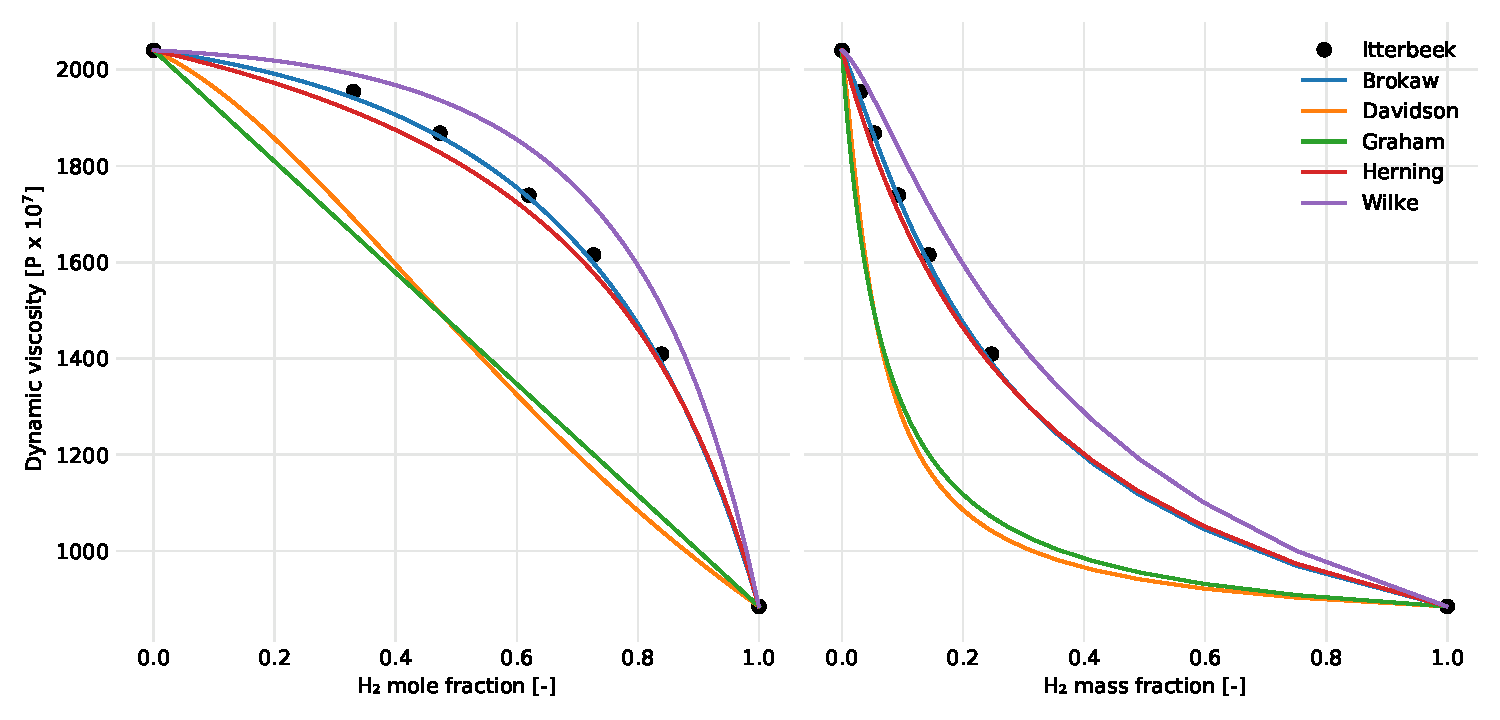
\includegraphics[width=\textwidth]{figures/gas-mu-h2o2-validate.pdf}
    \caption{Viscosity of a H$_2$/O$_2$ mixture at 293.6 K (20$^\circ$C). Calculated values represented by line profiles. Experiment data points from \cite{Itterbeek-1947} shown as symbols.}
    \label{fig:gas-mu-h2o2-validate}
\end{figure}

Properties for molecular weight, viscosity, and density for the gas mixtures investigated in this paper are shown in Figure \ref{fig:mix-properties}. Similar to the individual gas properties, the mixture properties were calculated at 101,325 Pa and 773.15 K (500$^\circ$C). The viscosity of the gas mixture was determined using the Herning and Zipperer method (Equation \ref{eq:herning}). The mole fraction of each gas in the mixture is given by the values shown at the top of each column in the figure. For example, the nitrogen and hydrogen mixture is comprised of 22\% nitrogen and 78\% hydrogen which is labeled as $0.22 + 0.78$. As expected, the carbon dioxide mixture is the heaviest in terms of molecular weight and density while the nitrogen and hydrogen mixture is the lightest. The most viscous mixture is the nitrogen and carbon monoxide where as the hydrogen mixtures are the least viscous.

\begin{figure}[H]
    \centering
    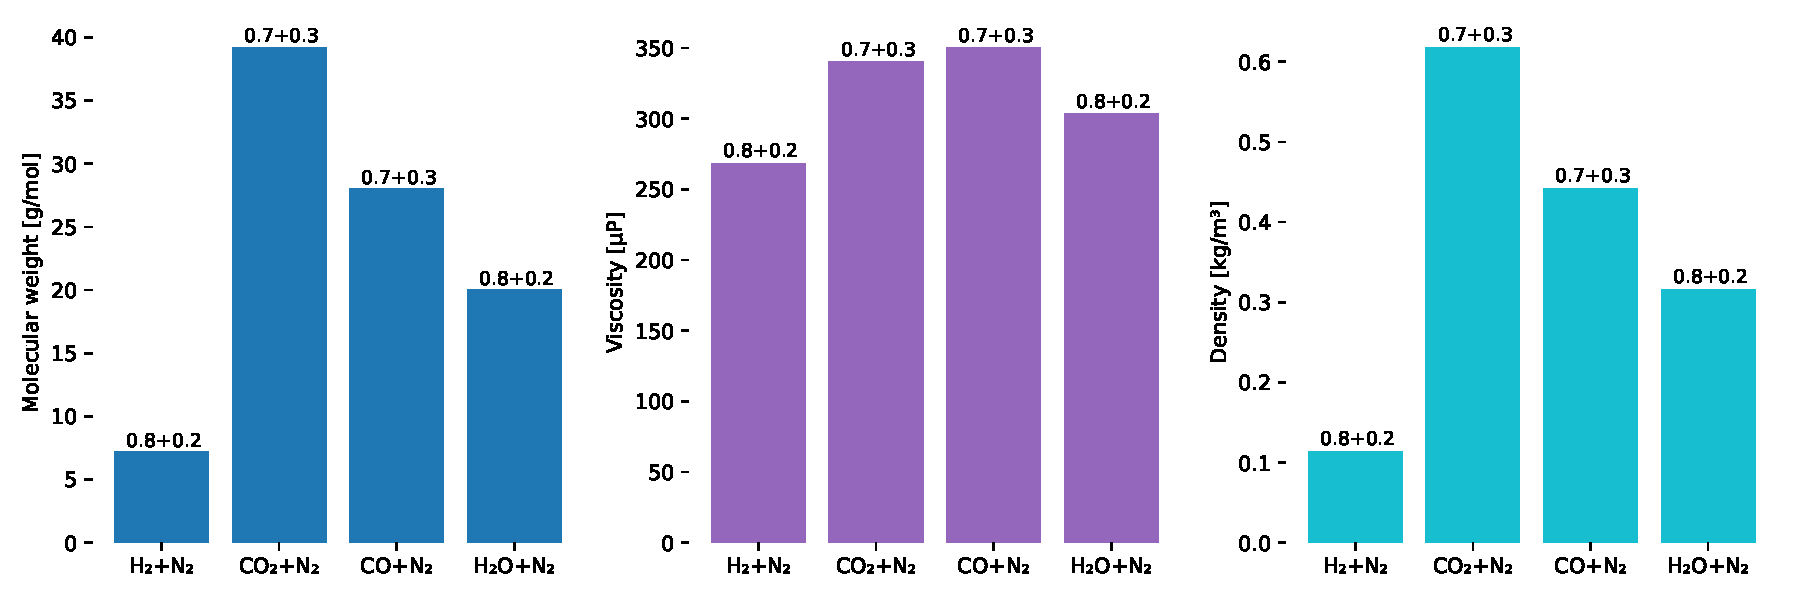
\includegraphics[width=\textwidth]{mix-properties.pdf}
    \caption{Comparison of gas mixture properties for molecular weight, viscosity, and density at 101,325 Pa and 773.15 K. Mole fraction of each gas component is shown at the top of each column.}
    \label{fig:mix-properties}
\end{figure}

% ----------------------------------------------------------------------------

\subsection{Fluidization characteristics}\label{sec:fluidization-charact}

Minimum fluidization velocity (U$_\text{mf}$) of the bed material for the different fluidization gases is presented in Table \ref{tab:umf-sand}. Hydrogen requires about twice the gas velocity to fluidize the bed of sand compared to the nitrogen, carbon monoxide, and carbon dioxide gases. This is due to hydrogen's lower viscosity and much lower density compared to the other gases. Water vapor and methane require moderately higher fluidization velocities compared to the nitrogen gas. A comparison of U$_\text{mf}$ for the various fluidization gases is displayed in Figure \ref{fig:umf-usumf-gases}.

\begin{table}[H]
    \centering
    \caption{Minimum fluidization velocity (m/s) of the bed material calculated from various correlations for different fluidization gases. Last row represents the average U$_\text{mf}$ value for each gas.}
    \label{tab:umf-sand}
    \begin{tabular}{lrrrrrr}
        \toprule
        U$_\text{mf}$ & N$_2$ & H$_2$ & H$_2$O & CO & CO$_2$ & CH$_4$ \\
        \midrule
        Ergun         & 0.14 & 0.30 & 0.18 & 0.15 & 0.16 & 0.23 \\
        Grace         & 0.10 & 0.21 & 0.13 & 0.11 & 0.11 & 0.16 \\
        Richardson    & 0.10 & 0.20 & 0.12 & 0.10 & 0.11 & 0.15 \\
        Wen and Yu    & 0.08 & 0.17 & 0.11 & 0.09 & 0.09 & 0.13 \\
        average       & 0.11 & 0.22 & 0.14 & 0.11 & 0.12 & 0.17 \\
        \bottomrule
    \end{tabular}
\end{table}

The superficial gas velocity (U$_\text{s}$) of the nitrogen gas flow is calculated as 0.3072 m/s which is based on the 14 SLM gas flow through the distributor plate. Using this value, the ratio of U$_\text{s}$ to U$_\text{mf}$ is shown in Table \ref{tab:us-umf-ratio} for different fluidization gases. The BFB pyrolysis reactor at NREL typically operates at a U$_\text{s}$/U$_\text{mf}$ of 3 with nitrogen gas. For gases such as H$_2$, H$_2$O, CO, CO$_2$, and CH$_4$, the gas flow into the reactor must be increased to have similar fluidized bed characteristics as the nitrogen case. A comparison of the increased U$_\text{s}$ for each gas along with the associated U$_\text{s}$/U$_\text{mf}$ is shown in Figure \ref{fig:us-usumf-gases}. As expected, the hydrogen gas flow must be approximately doubled compared to the nitrogen case to achieve similar fluidization of the bed material.

\begin{table}[H]
    \centering
    \caption{Ratio of U$_\text{s}$ to U$_\text{mf}$ for different fluidization gases. Last row represents the average U$_\text{s}$/U$_\text{mf}$ value for each gas.}
    \label{tab:us-umf-ratio}
    \begin{tabular}{lrrrrrr}
        \toprule
        U$_\text{s}$/U$_\text{mf}$ & N$_2$ & H$_2$ & H$_2$O & CO & CO$_2$ & CH$_4$ \\
        \midrule
        Ergun                      & 2.13 & 1.04 & 1.67 & 2.02 & 1.97 & 1.34 \\
        Grace                      & 2.99 & 1.47 & 2.35 & 2.84 & 2.76 & 1.88 \\
        Richardson                 & 3.16 & 1.55 & 2.48 & 3.00 & 2.91 & 1.98 \\
        Wen and Yu                 & 3.69 & 1.82 & 2.90 & 3.50 & 3.39 & 2.32 \\
        average                    & 2.99 & 1.47 & 2.35 & 2.84 & 2.76 & 1.88 \\
        \bottomrule
    \end{tabular}
\end{table}

\begin{figure}[H]
    \centering
    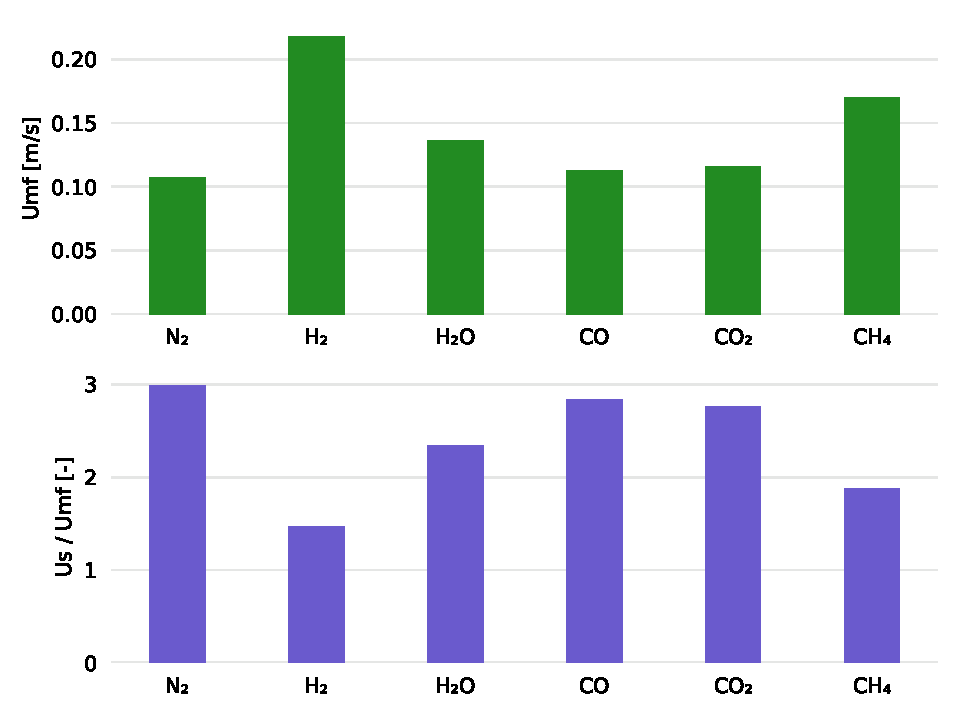
\includegraphics[width=0.8\textwidth]{figures/umf-usumf-gases.pdf}
    \caption{Comparison of the minimum fluidization velocity (U$_\text{mf}$) and the ratio of U$_\text{s}$/U$_\text{mf}$ for different fluidization gases. Superficial gas velocity is U$_\text{s}$.}
    \label{fig:umf-usumf-gases}
\end{figure}

\begin{figure}[H]
    \centering
    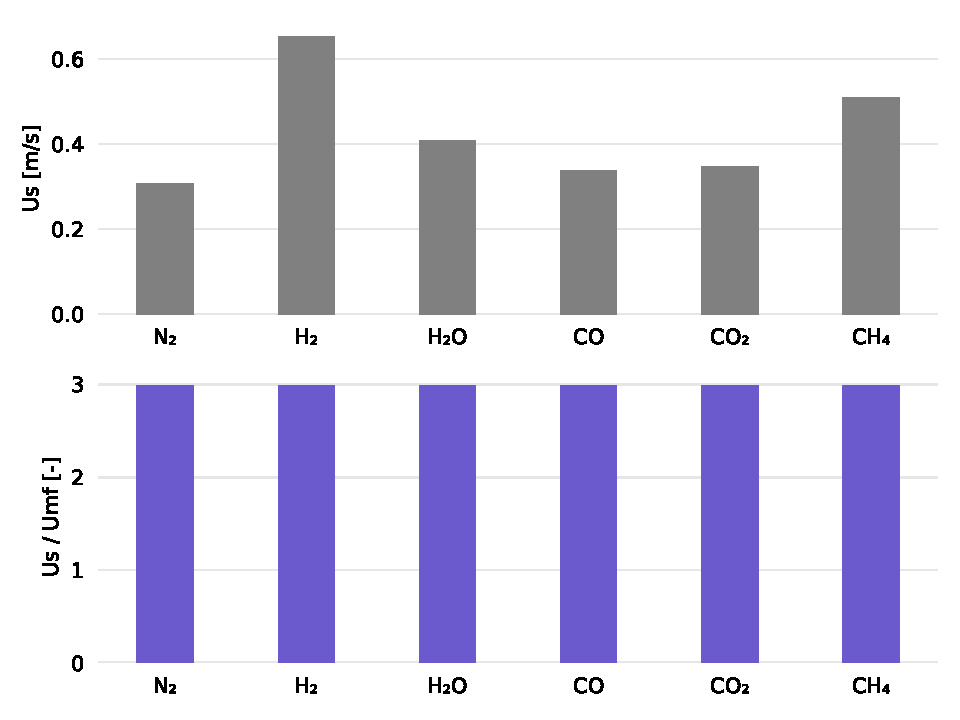
\includegraphics[width=0.8\textwidth]{figures/us-usumf-gases.pdf}
    \caption{Comparison of the superficial gas velocity (U$_\text{s}$) and the associated U$_\text{s}$/U$_\text{mf}$ for different fluidization gases. Minimum fluidization velocity is U$_\text{mf}$.}
    \label{fig:us-usumf-gases}
\end{figure}

The Reynolds number was calculated using an average biomass particle diameter of 369.4 $\mu$m and the mean U$_\text{mf}$ value. Next, the Nusselt number along with the associated convective heat transfer coefficient were calculated for each carrier gas as shown in Table \ref{tab:biomass-hconv} and Figure \ref{fig:biomass-hconv}. The highest heat transfer coefficient is estimated for H$_2$ while the second highest result is for CH$_4$. This is largely due to the higher thermal conductivity of the hydrogen and methane compared to the other gases. Due to the higher heat transfer rate to the biomass particle in the hydrogen environment, one can expect the biomass to pyrolyze more quickly with the hydrogen carrier gas.

\begin{table}[H]
    \centering
    \caption{Comparison of the Reynolds number, Nusselt number, and convective heat transfer coefficient (h) for different fluidization gases.}
    \label{tab:biomass-hconv}
    \begin{tabular}{lrrrr}
        \toprule
        Gas & U$_\text{mf}$ & Re & Nu & h \\
        \midrule
        N$_2$  & 0.11 & 0.48 & 2.55 & 369.45  \\
        H$_2$  & 0.22 & 0.14 & 2.26 & 2224.25 \\
        H$_2$O & 0.14 & 0.50 & 2.56 & 464.54  \\
        CO     & 0.11 & 0.53 & 2.58 & 389.53  \\
        CO$_2$ & 0.12 & 0.89 & 2.81 & 399.83  \\
        CH$_4$ & 0.17 & 0.70 & 2.69 & 862.61  \\
        \bottomrule
    \end{tabular}
\end{table}

\begin{figure}[H]
    \centering
    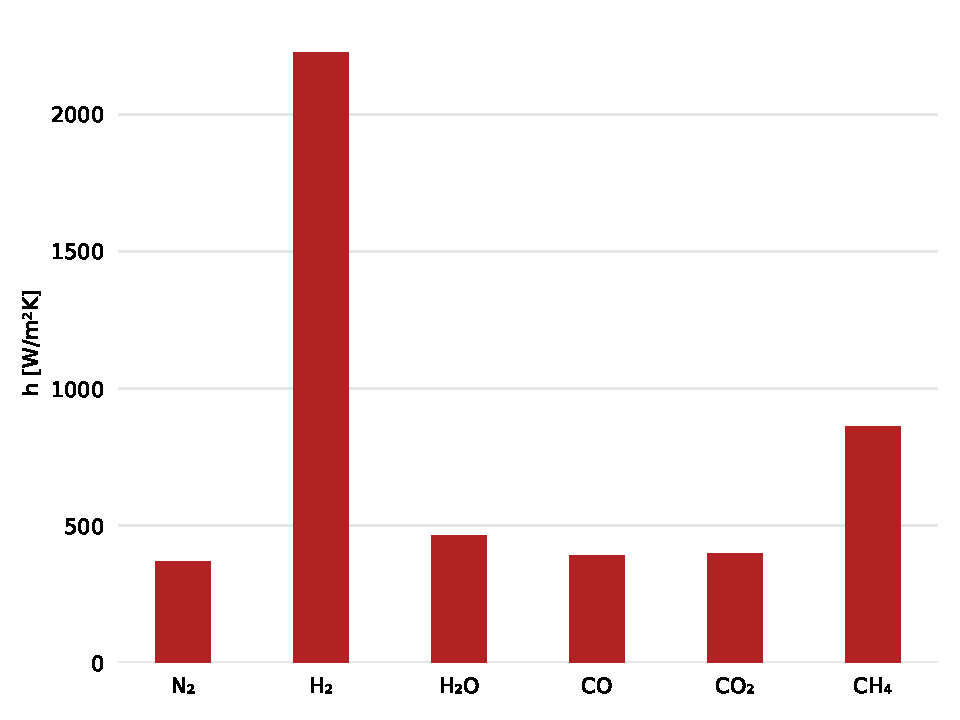
\includegraphics[width=0.8\textwidth]{figures/biomass_hconv.pdf}
    \caption{Convective heat transfer coefficient (h) for different fluidization gases. Values based on average biomass particle size and average minimum fluidization velocity.}
    \label{fig:biomass-hconv}
\end{figure}

% ----------------------------------------------------------------------------

\subsection{Evaluation of the kinetic scheme}

The Di Blasi kinetics were put to use in a batch reactor model to investigate the time scales associated with the reaction mechanisms. Figure \ref{fig:batch-blasi} is an overview of the biomass conversion and pyrolysis yields using the Di Blasi kinetics in a batch reactor at 773.15 K (500$^\circ$C). At this temperature, without the effects of secondary reactions, the kinetics offer a maximum achievable tar yield of 78\% within 5 seconds. However, if secondary reactions occur during the entire pyrolysis process then a maximum tar yield of only 53\% is possible. Modifying the pre-factor term for reaction 4 by a factor of 0.2, decreases the gas yield while increasing tar and char yields. The Di Blasi kinetics suggest that minimizing the extent of secondary reactions is critical to producing the maximum possible tar yield.

A range of reaction temperatures were applied to the Di Blasi kinetics in the batch reactor model as shown in Figure \ref{fig:batch-blasi-temps}. The kinetics suggest that temperature can increase the rate of primary tar production while decreasing devolatilization time. When secondary reactions occur during the entire pyrolysis process, maximum tar yields are realized at higher temperatures but with shorter residence times. These results suggest that if secondary reactions are minimized then maximum tar yield can be achieved within an appropriate residence time.

\begin{figure}[H]
    \centering
    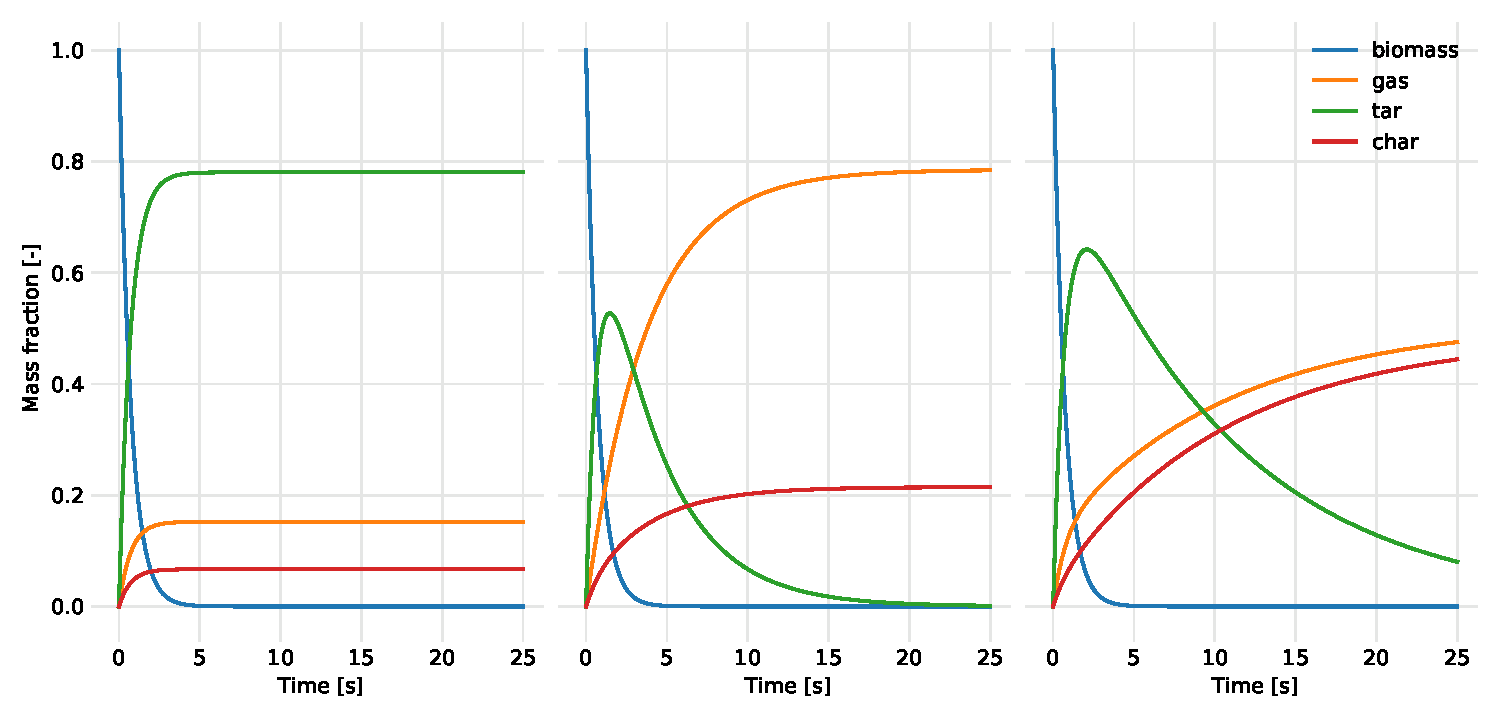
\includegraphics[width=\textwidth]{batch-blasi.pdf}
    \caption{Biomass conversion and product yields in a batch reactor model at 773.15 K (500$^\circ$C) according to the Di Blasi kinetic reactions. Primary reactions only (left). Primary and secondary reactions (center). Primary and secondary reactions using modified reaction 4 (right).}
    \label{fig:batch-blasi}
\end{figure}

\begin{figure}[H]
    \centering
    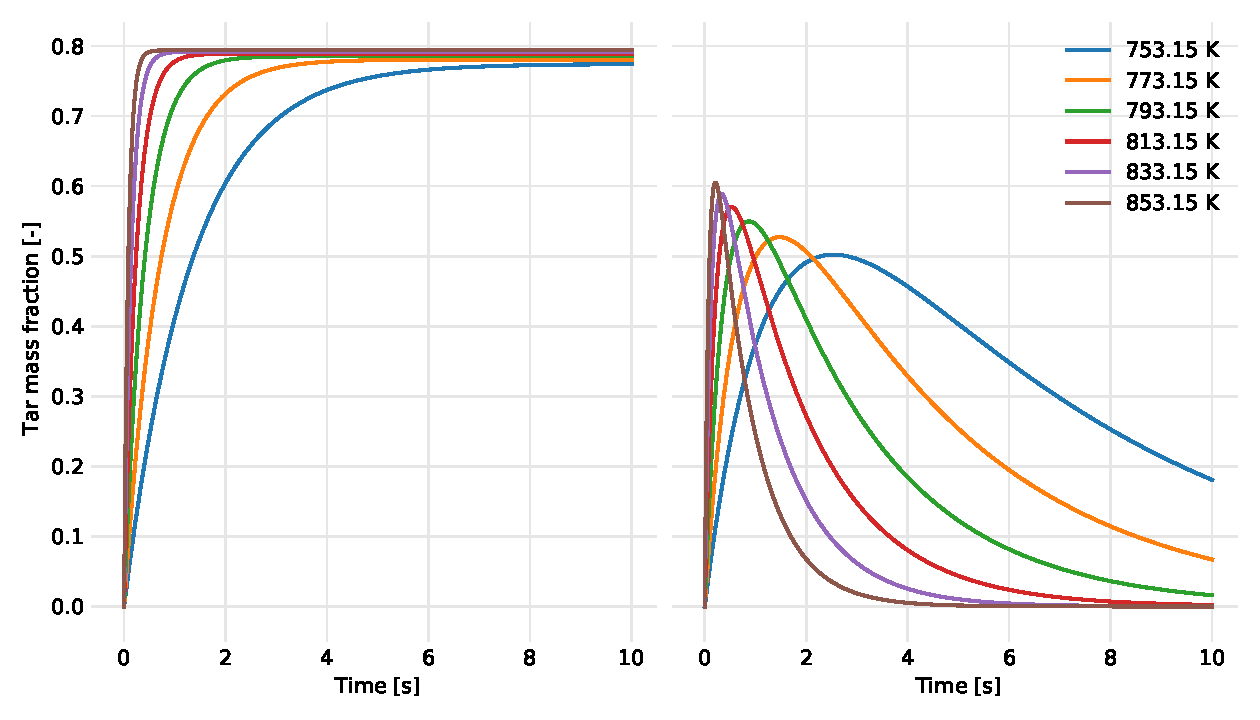
\includegraphics[width=\textwidth]{batch-blasi-temps.pdf}
    \caption{Tar yields for reaction temperatures of 753.15--853.15 K (480--580$^\circ$C) using the Di Blasi kinetics in a batch reactor model. Results shown for primary tar (left) along with primary and secondary tar (right).}
    \label{fig:batch-blasi-temps}
\end{figure}

% ----------------------------------------------------------------------------

\subsection{Limiting factors for biomass pyrolysis}

Gas influence on the pyrolysis limiting regimes is shown in Figure \ref{fig:biot-pyro-gases} for a biomass particle diameter of 369.4 $\mu$m. The regime map suggests that gas properties have little effect on the limiting mode of pyrolysis. However, when comparing a range of particle diameters, the differences are more pronounced as seen in Figure \ref{fig:biot-pyro-diams}. For larger particles, conduction becomes the limiting mode of pyrolysis especially for the hydrogen gas. For smaller particles, nitrogen gas promotes isothermal conditions along with a kinetically limited regime.

\begin{figure}[H]
    \centering
    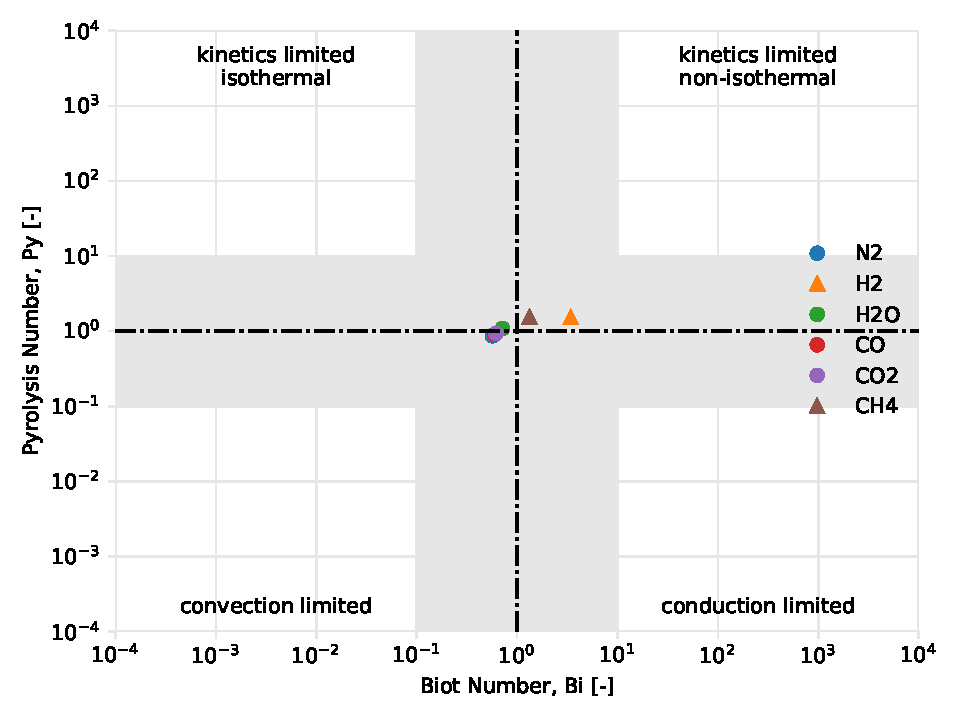
\includegraphics[width=0.8\textwidth]{figures/biot-pyro-gases.pdf}
    \caption{Comparison of carrier gas effects on pyrolysis regime for a 369.4 $\mu$m biomass particle. Grey region means no dominant mechanism controlling pyrolysis.}
    \label{fig:biot-pyro-gases}
\end{figure}

\begin{figure}[H]
    \centering
    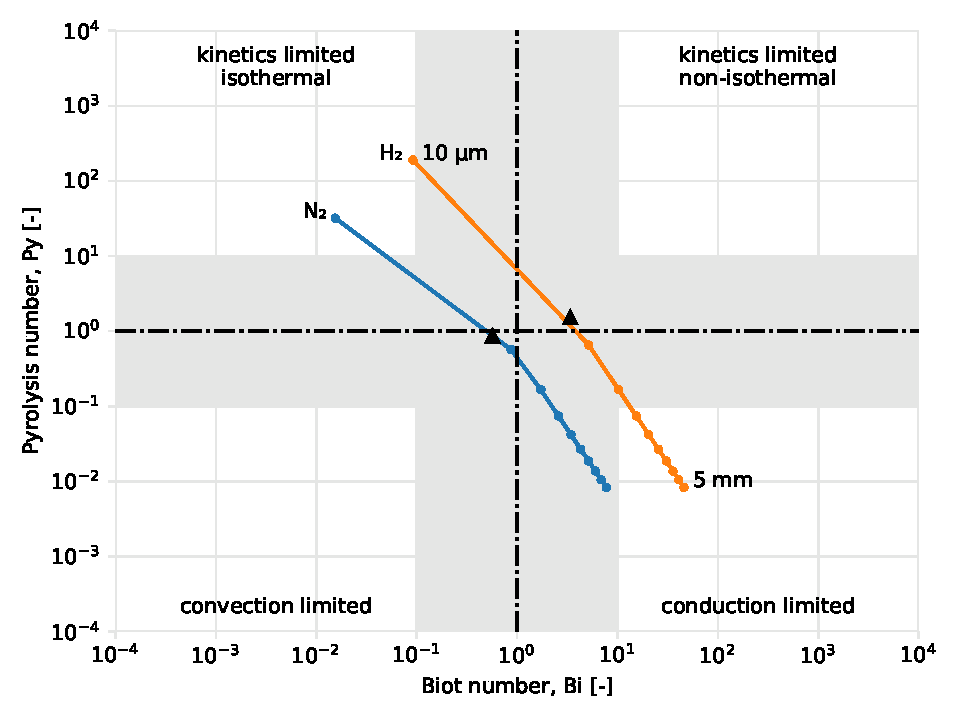
\includegraphics[width=0.8\textwidth]{figures/biot-pyro-diams.pdf}
    \caption{Comparison of nitrogen and hydrogen gas effects for biomass particles ranging from 10$\mu$m to 5 mm in diameter. Triangle markers symbolize 369.4 $\mu$m biomass particle diameter. Grey region means no dominant mechanism controlling pyrolysis.}
    \label{fig:biot-pyro-diams}
\end{figure}

% ----------------------------------------------------------------------------

\subsection{CFD-DEM validation}

The predicted yield of pyrolysis products (bio-oil, light gases, and biochar) was validated against experimental data of biomass pyrolysis using the same NREL 2FBR reactor system that was modeled and simulated in this work \cite{French-2021}. The process variables used in the experimental work are consistent with those implemented for the N$_2$ and H$_2$ cases (run ID = 1 and 2, respectively). The mass closure of the experimental data was about 94\%, therefore a mass proportional modification of the original data was performed to enforce 100\% mass closure and form a proper basis of comparison to the CFD--DEM simulation predictions. Table \ref{tab:cfddem-validation} shows that the predicted yields of pyrolysis products closely follow the experimental data. The magnitude of the relative prediction deviation ranged between 0.1\% and 9.0\%.

The prediction performance of the CFD--DEM model was highest for bio-oil, with a maximum absolute relative deviation of 1\%. The light gas yield for the N$_2$ case was overpredicted relative to the eperimental data, whereas the inverse was found for the H$_2$ case, where light gas was underpredicted. Similarly, biochar was slightly overpredicted for the H$_2$ but underpredicted for the N$_2$ case.

\begin{table}[H]
    \centering
    \caption{CFD–DEM model validation against experimental data. Product yields were calculated on a biomass weight basis. Experiment data from \cite{French-2021}.}
    \label{tab:cfddem-validation}
    \begin{tabular}{cccccc}
        \toprule
               & Fluidizing   & Pyrolysis & \multicolumn{2}{c}{Pyrolysis yield (wt.\%)} & Relative \\
        Run ID & gas          & product   & Experiment & Simulation                     & deviation (\%) \\
        \midrule
        1 & N$_2$ & bio-oil   & 74.5      & 74.5       & 0.1     \\
        1 & N$_2$ & light gas & 12.3      & 13.4       & 9.0     \\
        1 & N$_2$ & biochar   & 13.2      & 12.1       & --8.6   \\
        2 & H$_2$ & bio-oil   & 73.7      & 74,5       & 1.0     \\
        2 & H$_2$ & light gas & 15.0      & 13.8       & --7.8   \\
        2 & H$_2$ & biochar   & 11.3      & 11.7       & 3.6     \\
        \bottomrule
    \end{tabular}
\end{table}

% \subsection{Fluidizing gas effect on pyrolysis performance at a constant flow rate/velocity (U$_s$)}
\subsection{Fluidizing gas effect on pyrolysis performance at a constant flow rate/velocity (U\texorpdfstring{$_s$}{s})}

The yields of pyrolysis bio-oil, light gas, and biochar for the different fluidizing gases at a constant flow rate of 14 SLPM ($6.61\times10^{-4}$ m$^3$/s) are compared in Figure \ref{fig:cfd-product-yield}. The observed differences in the pyrolysis product distribution among the fluidizing gases were minimal. The highest bio-oil yield of 74.8 wt.\% and lowest bio-oil yield of 73.8 wt.\% were obtained when pure CH$_4$ and CO were used as fluidizing gas, respectively. The bio-oil yield was slightly higher when any of H$_2$, CH$_4$, and CO$_2$ replaced N$_2$ as the fluidizing gas. The evidence reviewed here suggests that light gas may be recirculated at a constant flow rate during pyrolysis without causing substantial losses in bio-oil yield.

\begin{figure}[H]
    \centering
    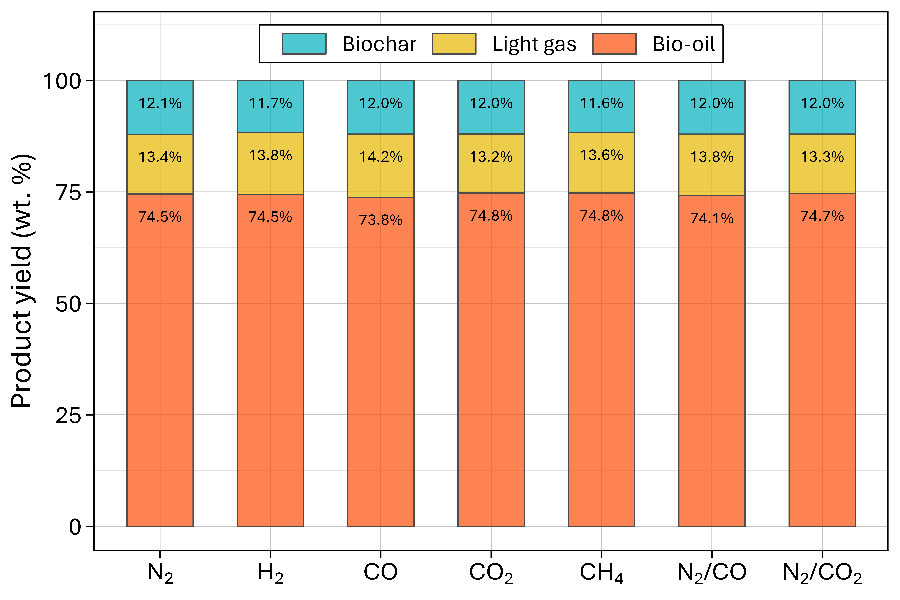
\includegraphics[width=1.0\textwidth]{figures/cfd-product-yield.pdf}
    \caption{Pyrolysis product distributions for different fluidizing gas at a constant flow rate. Product yields were calculated on a biomass weight basis.}
    \label{fig:cfd-product-yield}
\end{figure}

A summary of the particle residence time for each fluidizing gas considered is given in Table \ref{tab:particle-restime}. It was unsurprising to find that the median particle residence time increased with increasing initial diameter of the biomass particles. The difference in particle residence time among the fluidizing gases also generally increased with increasing initial diameter of biomass particles. In other words, the impact of fluidizing gas on particle residence time is stronger for larger particles and weaker for smaller particles.

\begin{table}[H]
    \centering
    \caption{Particle residence time of biomass particle for different fluidizing gas at a constant flow rate and different initial particle diameter where d$_p$ is initial biomass particle diameter.}
    \label{tab:particle-restime}
    \begin{tabular}{cccccc}
        \toprule
               & Fluidizing & \multicolumn{4}{c}{Median particle residence time (s)} \\
        Run ID & gas        & d$_p$ = 296 $\mu m$ & d$_p$ = 333 $\mu m$ & d$_p$ = 371 $\mu m$ & d$_p$ = 408 $\mu m$ \\
        \midrule
        1 & N$_2$        & 6.8 & 8.7  & 11.1  & 14.3 \\
        2 & H$_2$        & 9.5 & 14.4 & 18.4 & 21.1 \\
        3 & CO           & 6.9 & 8.9  & 11.0  & 14.1 \\
        4 & CO$_2$       & 6.3 & 7.9  & 10.5  & 12.5 \\
        5 & CH$_4$       & 7.3 & 10.5  & 14.1 & 18.1 \\
        6 & N$_2$/CO     & 6.8 & 9.0  & 12.2  & 14.3 \\
        7 & N$_2$/CO$_2$ & 6.5 & 8.2  & 10.0  & 12.9 \\
        \bottomrule
    \end{tabular}
\end{table}

Figure \ref{fig:cfd-temp-void-biooil} shows the gas phase temperature, void volume fraction, and bio-oil degradation rates profile along the reactor height for different fluidizing gas at a constant flow rate. The gas-phase temperature was higher in the freeboard than in the bed. This is attributed to the fact that enthalpy for biomass pyrolysis reactions is drawn from inside the bed because pyrolysis reactions occur predominantly inside the bed. Additionally, the gas temperature was relatively unchanged along the reactor height within the bed whereas, in the freeboard, the gas temperature increased towards the reactor outlet. Also noteworthy is the fact that the gas temperature along the reactor height was consistently highest when H$_2$ was used as fluidizing gas (Figure \ref{fig:cfd-temp-void-biooil}a). This observation is attributable to the large difference in the thermal conductivity of H$_2$ compared to the other fluidization gases (Figure \ref{fig:gas-properties}). It should be noted that the difference observed in the fluid temperature was less than 10$^{\circ}$C. The average height of the fluidized bed was about 0.14 m for all the fluidizing gases considered, except for H$_2$ and CH$_4$ which produced a lower bed height (Figure \ref{fig:cfd-temp-void-biooil}b). The bed height was determined as the position along the reactor height where the void volume fraction approached 0.7.

\begin{figure}[H]
    \centering
    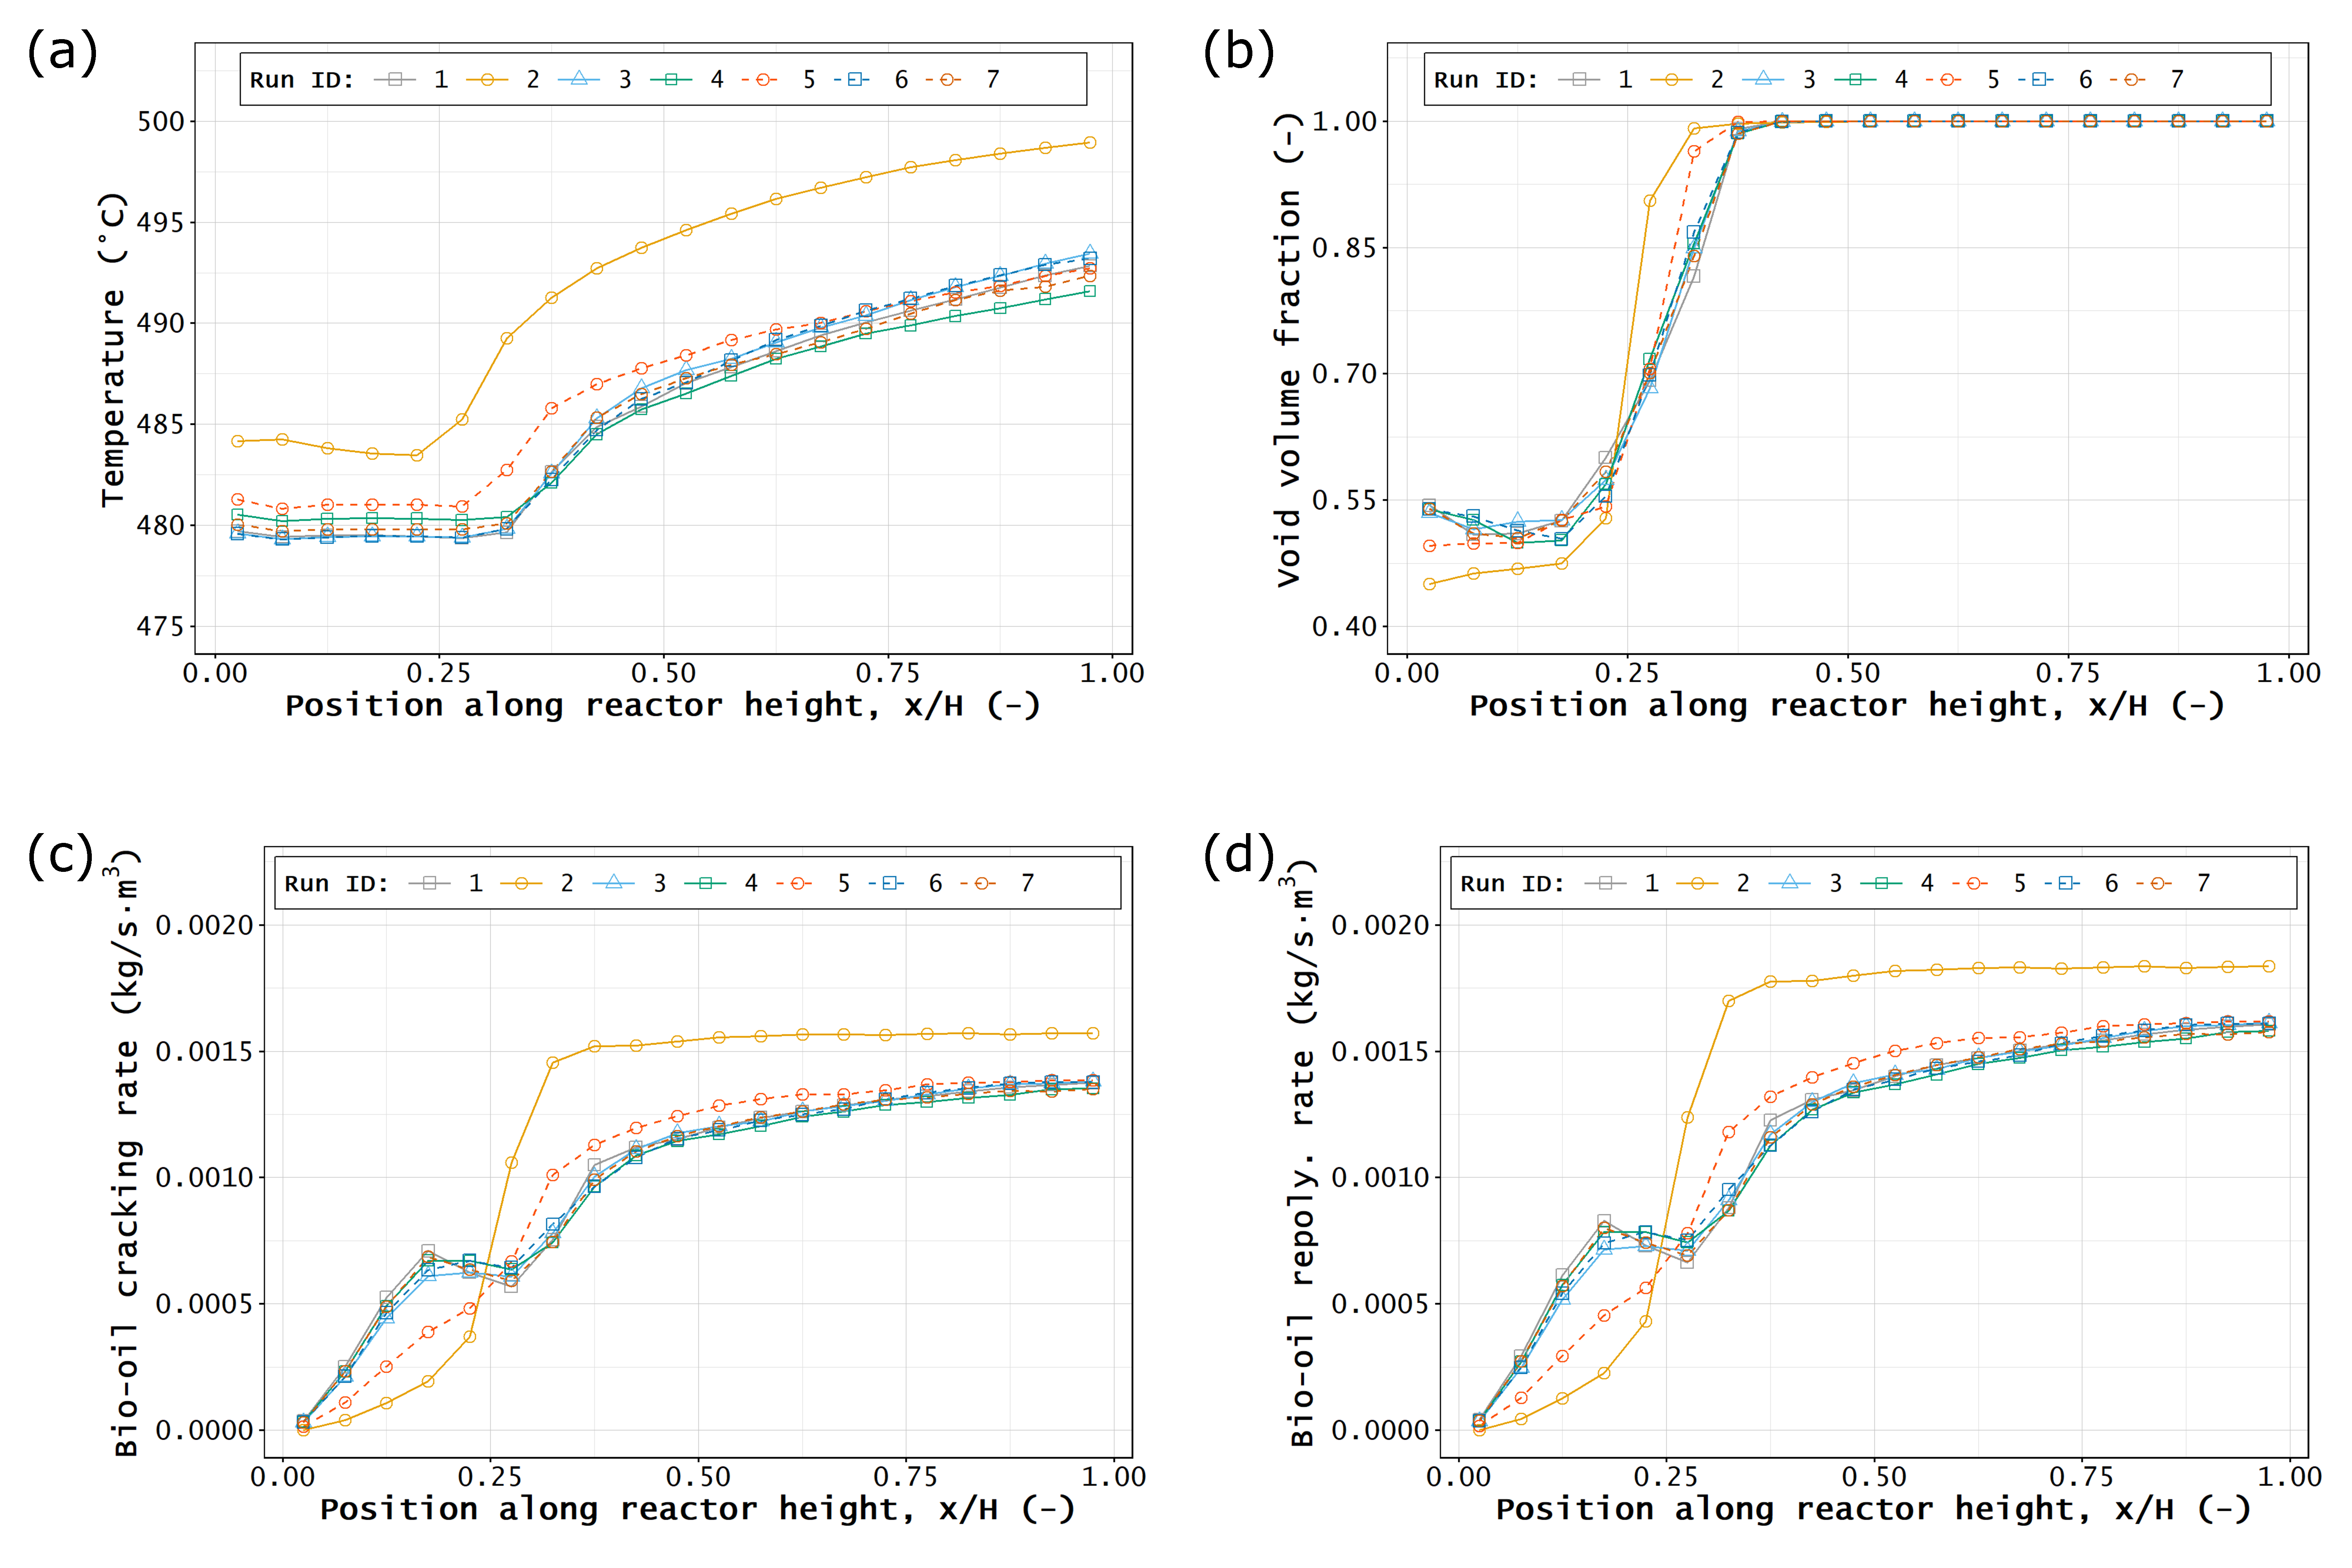
\includegraphics[width=1.0\textwidth]{figures/cfd-temp-void-biooil.pdf}
    \caption{Profile of (a) fluid temperature, (b) fluid volume fraction, (c) bio-oil cracking reaction rate, (d) bio-oil repolymerization reaction rate along the reactor height for different fluidizing gas at a constant flow rate. The reactor height (0.43 m) is denoted by the letter H.}
    \label{fig:cfd-temp-void-biooil}
\end{figure}

The observed degradation rates for both the particle and vapor phases were substantially affected by the fluidizing gas used. The shape of the bio-oil cracking rate profile along the reactor height was similar to that of the bio-oil repolymerization rate for all the fluidizing gases considered (Figure \ref{fig:cfd-temp-void-biooil}c and Figure \ref{fig:cfd-temp-void-biooil}d). Bio-oil degradation rates were higher in the freeboard than in the bed. The overall bio-oil degradation rates with H$_2$ as the fluidizing gas were substantially higher than those observed with other fluidizing gases. The reactor volume-averaged bio-oil cracking and repolymerization rates were $1.31\times10^{-3}$ and $1.54\times10^{-3}$ kg/s·m$^3$ for H$_2$, respectively $1.21\times10^{-3}$ and $1.42\times10^{-3}$ kg/s·m$^3$ for N$_2$, respectively. This data demonstrates that bio-oil degradation rates were 8\% higher when H$_2$ replaced N$_2$ as the fluidizing gas. This observation explains the reason why despite H$_2$ yielding the highest particle heating and mass-loss rates (Figure \ref{fig:cfd-masspercent}), and one of the longest residence times (Table \ref{tab:particle-restime}), its bio-oil yield is marginally different from the bio-oil yield with other fluidizing gases, especially N$_2$. When H$_2$ was used as fluidizing gas, biomass particles experienced significantly higher heating rates, and consequently higher mass-loss rates, compared to when other fluidizing gases were used. The impact of fluidizing gas on the heating and mass-loss rates was higher for larger particles. Generally, biomass heating and mass-loss rates follow the order: H$_2$ $>$ CH$_4$ $>$ CO $>$ N$_2$ $>$ N$_2$/CO $>$ N$_2$/CO$_2$ $>$ CO$_2$ which correlates well with the effective thermal conductivity of the fluidizing gas.

\begin{figure}[H]
    \centering
    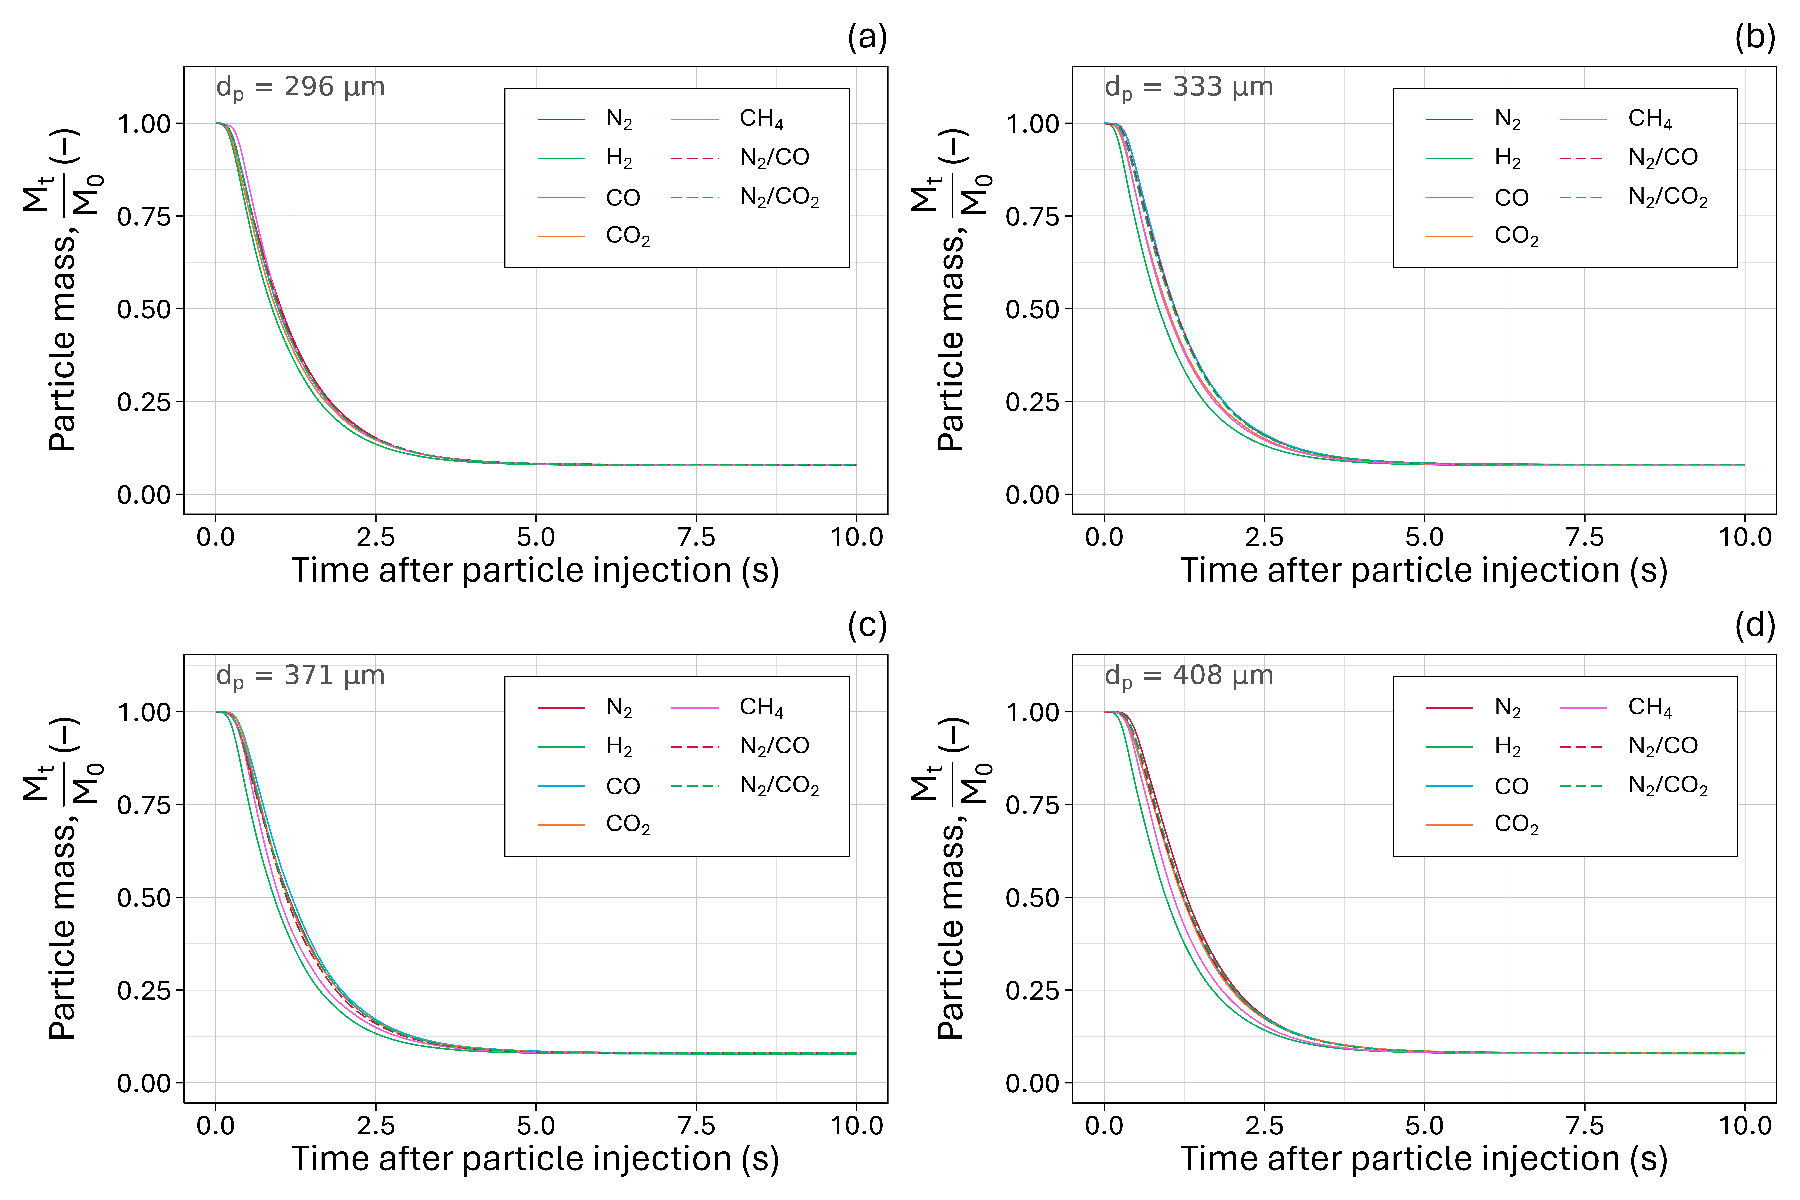
\includegraphics[width=1.0\textwidth]{figures/cfd-masspercent.pdf}
    \caption{Average biomass particle thermogravimetry curve for different fluidizing gas at a constant flow rate (a) nominal particle size = 296 $\mu m$, (b) nominal particle size = 333 $\mu m$, (c) nominal particle size = 371 $\mu m$, and (d) nominal particle size = 408 $\mu m$.}
    \label{fig:cfd-masspercent}
\end{figure}

Overall, the model results indicate that light gas produced during pyrolysis can be recirculated as fluidizing gas at a constant flow rate without detrimental consequences on pyrolysis performance. Additionally, we demonstrated that fluidizing gas can notably increase biomass heating and mass-loss rates (pyrolysis conversion rate). This suggests potential process intensification implications because heating and mass-loss rates represent a major bottleneck in conventional pyrolysis systems. Achieving increased heating and mass-loss rates may lead to significant improvement in process throughput and scaleup.

\subsection{Fluidizing gas effect on pyrolysis performance with constant fluidization number (\texorpdfstring{U$_\text{s}$/U$_\text{mf}$}{Us/Umf})}

As discussed in Section \ref{sec:fluidization-charact}, the value of U$_\text{s}$/U$_\text{mf}$ varies for each fluidizing gas composition when the flowrate is kept constant. As a result, the dynamic behavior of the bed, which U$_\text{s}$/U$_\text{mf}$ characterizes, varies with the gas composition. These differences are most pronounced between N$_2$ and H$_2$ which have U$_\text{s}$/U$_\text{mf}$ values of ~3.0 and ~1.5, respectively, when U$_\text{s}$ remains constant. To investigate the effect of gas properties on pyrolysis yields, the mass fraction of H$_2$ was varied between 0 and 1 (with the N$_2$ as the remaining fraction) while maintaining a constant U$_\text{s}$/U$_\text{mf}$ = 3.0. Figure \ref{fig:cfd-constuumf-particle-temp-density} shows the average particle temperature and mass as a function of time after injection into the reactor for each particle size in both N$_{2}$ and H$_{2}$ fluiding gas streams. Here it can be seen, as for the constant $U_\text{s}$ case, the larger heat transfer coefficient associated with the H$_2$ fluidizing gas (h$_{\text{H}_2}$ = 2224.3, h$_{\text{N}_2}$ = 368.5 W/m$^2$K) result in greater rates of heat transfer and mass loss. Additionally, the nearly identical time distributions of the particle temperature and mass for H$_2$ with constant U$_\text{s}$ and U$_\text{s}$/U$_\text{mf}$ indicates that total heat transfer to a particle in bubbling fluidized bed is independent of the gas velocity. This is consistent with previous results that while convection increases with gas velocity, this increase is offset by decreases in conduction between solids in the bed \cite{Collier-2004,zhou2009particle}.

\begin{figure}[H]
    \centering
    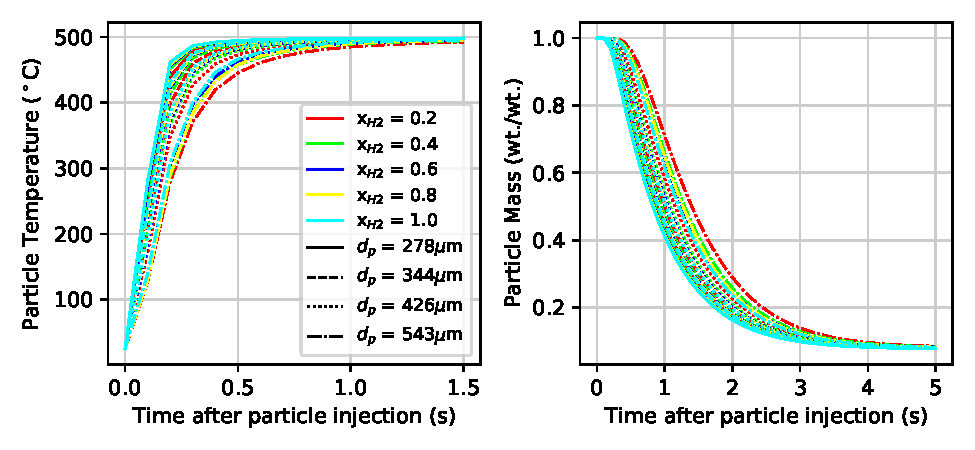
\includegraphics[width=\textwidth]{figures/cfd-constuumf-particle-temp-density.pdf}
    \caption{Average particle temperature (left) and density (right) as a function of residence time in reactor for N$_2$ and H$_2$ carrier gasses. For H$_2$ carrier gas, results with both constant U$_\text{s}$ and U$_\text{s}$/U$_\text{mf}$ are provided.}
    \label{fig:cfd-constuumf-particle-temp-density}
\end{figure}

At the reactor conditions and particle sizes investigated, the gas velocities are insufficient for biomass particles to elutriate from the reactor at their initial density and diameter. Therefore, the particle remains in the reactor until its size and mass are sufficiently reduced by pyrolysis to be ejected from the reactor. This can be seen in Figure \ref{fig:cfd-constuumf-terminal-vel}, which contains the particle diameter and density at which the terminal velocity, U$_\text{t}$, is equal to the gas velocity for each H$_2$ mass fraction investigated. At the initial particle density, the maximum diameter at which U$_\text{s}$ $\ge$ U$_\text{t}$ falls well outside of the initial paticle distribution in all cases. As as result, the particles remain in the reactor, losing size and mass as biomass is converted to bio-oil and char until their their terminal velocity is sufficiently small for elutriation to occur. As discussed previously, the lower density of H$_2$ reduces the drag induced on the particles by the flow. As a result the, switching the working fluid from N$_2$ to H$_2$ results in a significant decrease in the maximum particle size at which U$_\text{s}$ = U$_\text{t}$ for a given particle density (348 and 345 $\mu$m for Y$_{\text{H}_2}$ = 0 and 156 and 214 $\mu$m for Y$_{\text{H}_2}$ = 1 at the initial and char densities, respectively). When the gas velocity is increased to maintain constant U$_\text{s}$/U$_\text{mf}$, the increased gas velocity offsets the effect of the lower density, resulting in smaller decreases in the maximum particle diameter at which U$_\text{t}$ = U$_\text{s}$ for a given density. Specifically, the maximum diameters differ by 20 $\mu$m at the initial density and 30 $\mu$m across range of H$_2$ mass fractions. This produces a similar effect on the similar particle residence times, which can be seen in Figure \ref{fig:cfd-constuumf-rtd}, which contains the average residence time for each particle diameter plotted against the H$_2$ mass fraction in the fluidizing gas. Here, we see that while the particle residence time increases with increasing mass fraction of H$_2$, this effect is more pronounced when U$_\text{s}$ is held constant. This is particularly true for the largest particle sizes with the average residence time increasing 19\% between Y$_{\text{H}_2}$ = 0 and Y$_{\text{H}_2}$ = 1 for constant U$_\text{s}$/U$_\text{mf}$ and 45\% for constant U$_\text{s}$.

\begin{figure}[H]
    \centering
    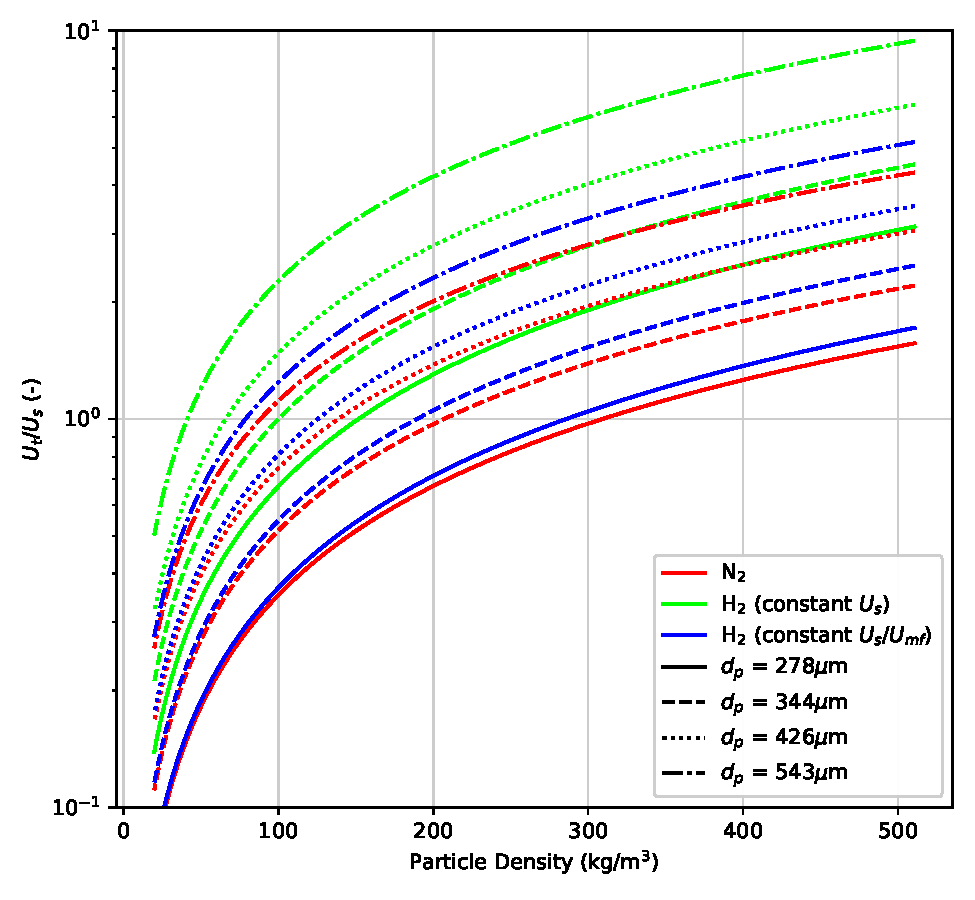
\includegraphics[width=0.8\textwidth]{figures/cfd-constuumf-terminal-vel.pdf}
    \caption{Particle diameter and density at which terminal velocity, U$_\text{t}$ is equal to the superficial gas velocity, U$_\text{s}$, for N$_2$ and H$_2$ carrier gasses. For H$_2$ carrier gas, results with both constant U$_\text{s}$ and U$_\text{s}$/U$_\text{mf}$ are provided.}
    \label{fig:cfd-constuumf-terminal-vel}
\end{figure}

\begin{figure}[H]
    \centering
    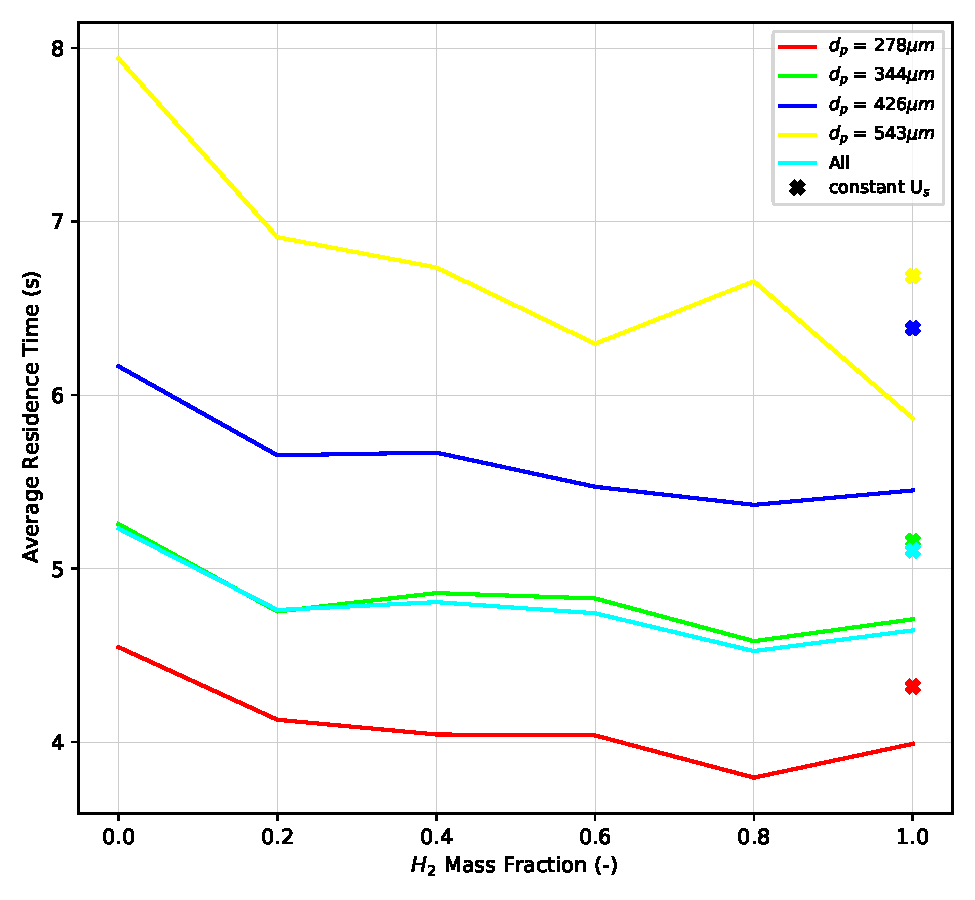
\includegraphics[width=0.8\textwidth]{figures/cfd-constuumf-rtd.pdf}
    \caption{Average particle residence time as a function of H$_2$ mass fraction in fluidizing gas at constant U$_\text{s}$/U$_\text{mf}$. Average residence times for H$_2$ fluidizing gas with constant U$_\text{s}$ indicated by markers in the plot.}
    \label{fig:cfd-constuumf-rtd}
\end{figure}

The effect of maintaining a constant U$_\text{s}$/U$_\text{mf}$ while increasing the mass fraction of H$_2$ in the fluidizing gas can be seen in Figure \ref{fig:cfd-constuumf-yields}, which contains plots of the product yields as well as the fraction of biomass converted for each gas composition and particle size. Because the particles must undergo significant mass loss and shrinkage before their terminal velocity is sufficiently low for elutriation, $>$99\% of the biomass is converted for all particle sizes and H$_2$ mass fractions investigated. For all particle sizes, the yields of light gasses and char decreased with increasing H$_2$ mass fraction with averages decreasing from 14.5\% to 13.3\% and 12.0\% to 10.6\%, respectively. These decreases in the char and light gas yields are accompanied by increases in the bio-oil yields, with the average increasing from 72.8\% in N$_2$ to 75.2\% in H$_2$. This increase is due to the low density of H$_2$ allowing for larger gas velocities without reducing the partice residence times. By maintaining similar residence times, the fraction of biomass converted to bio-oil remains constant while the higher gas velocities reduce the residence time of the resulting oil. The shorter residence time of the oil reduces the amount lost to secondary reactions converting it to char (repolymerization) and light gas (cracking). This can be seen in Figure \ref{fig:cfd-constuumf-reaction-rates} which shows the time and volume averaged cracking and repolymerization reaction rates in the reactor for each H$_2$ mass fraction. While maintaining a constant gas velocity when switching the fluidizing gas from N$_2$ to H$_2$ results in a slight increase in both secondary reactions, increasing the gas flowrate to maintain a constant U$_\text{s}$/U$_\text{mf}$ leads a decrease of 42.9\% in both the polymerization and cracking reaction rates. This results to the increased bio-oil production and subsequent decrease in light gas and char production when using H$_2$ as the fluidizing gas.

\begin{figure}[H]
    \centering
    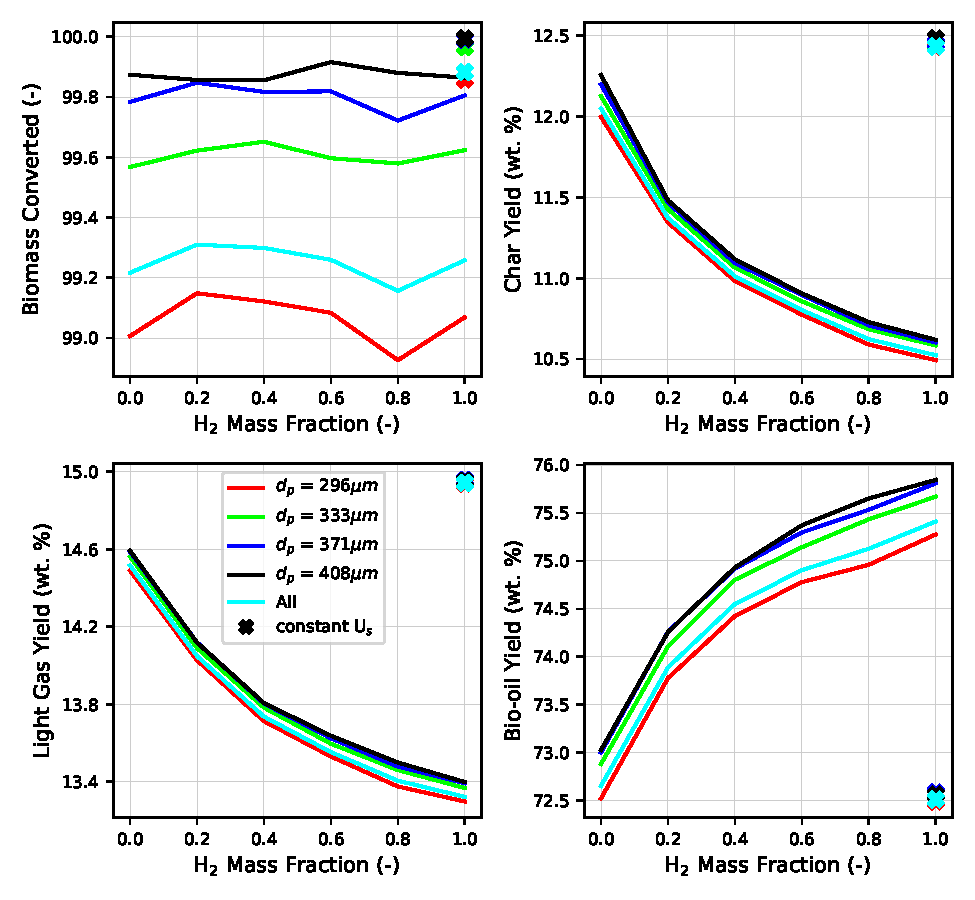
\includegraphics[width=\textwidth]{figures/cfd-constuumf-yields.pdf}
    \caption{Fraction of biomass converted and product yields as a function of H$_2$ mass fraction at constant U$_\text{s}$/U$_\text{mf}$. Biomass converted and product yields for H$_2$ fluidizing gas with constant U$_\text{s}$ indicated by markers in the plot.}
    \label{fig:cfd-constuumf-yields}
\end{figure}

\begin{figure}[H]
    \centering
    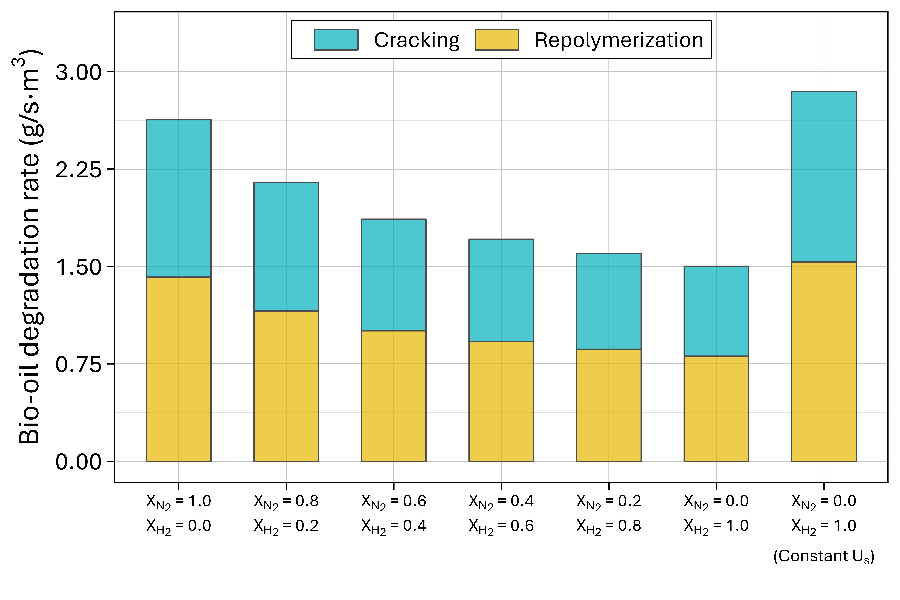
\includegraphics[width=1.0\textwidth]{figures/cfd-constuumf-reaction-rates.pdf}
    \caption{Volume and time averaged secondary reaction rates as a function of H$_2$ mass fraction at constant U$_\text{s}$/U$_\text{mf}$. Reaction rates with H$_2$ fluidizing gas and constant U$_\text{s}$ included for comparison.}
    \label{fig:cfd-constuumf-reaction-rates}
\end{figure}
